\section{ERCI as multi-objective optimization}\label{sec:convex}
We investigate the ERCI problem statement. Based on a sequence of observations, we reduce the ERCI problem to the Core ERCI problem which significantly eases the description (and implementation) of the algorithm afterwards.

\subsection{Preprocessing}
To ease the technical exposition, without loss of generality, we make
the following assumptions:
We assume the graph
structure underlying the SG is finite and acyclic -- and thus all paths
are finite length. When considering $\tau$-bounded path properties (monitorable by finite automata),
this assumption is naturally realized by a $\tau$-step unrolling of a
monitor augmented SG \footnotemark, i.e., augmenting the state space with a counter from $0$ to $\tau$ and the current property monitor state. 

\footnotetext{
One may then represent this unrolled graph as a binary
decision diagram, resulting in a (typically) concise graph that grows
proportional to the horizon and minimal state space augmentation
required~\cite{DBLP:conf/cav/Vazquez-Chanlatte20}.}

Next, in order to ensure the hard constraint, $\hard$, we
calculate all states from which the $\pTwo$-player can enforce
violating the hard constraint. Such states are identifiable using a single
topologically ordered pass over $\sg$ from the terminal states to the initial state.  We remove
such states along with their in- and outgoing transitions. Any
$\pOne$-policy now satisfies the hard constraint. 
The remaining terminal states are all merged into two states $\target$ and
$\sink$, based on membership in $\soft$, i.e.,
\begin{equation}
  \begin{split}
    \last{\path} = \target ~\implies~ \path \in \soft\\
    \last{\path} = \sink ~\implies~ \path \notin \soft
  \end{split}.
\end{equation}

\begin{example}
	In Fig.~\ref{fig:minimal:mdp} we show a (deterministic) MDP and we plot for all schedulers the induced probability to reach $\target$ and the induced causal entropy, in Fig.~\ref{fig:minimal:soft} and \ref{fig:minimal:entropy}, respectively. 
	We see that taking action $a$ with increasing probability yields a larger probability to reach $\target$, whereas taking action $a$ and~$b$ uniformly at random is optimal for the entropy. 
\end{example}


\begin{figure}
\centering
\begin{subfigure}{0.24\columnwidth}
\centering
\begin{tikzpicture}	
	\node[sstate,initial, initial text=] (si) {$s_0$};
	\node[tstate,above=0.6cm of si] (s0) {$\target$};
	\node[tstate,below=0.6cm of si] (s1) {$\sink$};
	\draw[->] (si) -- node[right] {$a$} (s0);
	\draw[->] (si) -- node[right] {$b$} (s1);
	
\end{tikzpicture}
\caption{Minimal MDP}
\label{fig:minimal:mdp}
\end{subfigure}
\begin{subfigure}{0.36\columnwidth}
\centering
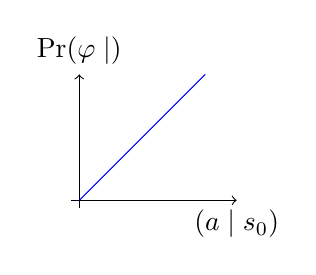
\begin{tikzpicture}[scale=2]
 \draw[->] (-0.05, 0) -- (1, 0) node[below]{$\sched(a \mid s_0 )$};
  	\draw[->] (0, -0.05) -- (0, 0.8) node[above] {$\Pr( \varphi \mid \sched)$};
  	%\draw[-,dashed] (0.4,0) -- (0.4,0.5184);
  	%\draw[-,dashed] (0.0,0.5184) -- (0.4,0.5184);
  \draw[ domain=0:0.8, smooth, variable=\x, blue] plot ({\x}, {\x});
\end{tikzpicture}
\caption{Probability to reach $\target$}
\label{fig:minimal:soft}
\end{subfigure}
\begin{subfigure}{0.36\columnwidth}
\centering
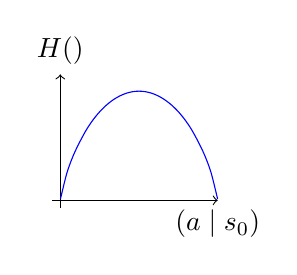
\begin{tikzpicture}[scale=2]	
 \draw[->] (-0.05, 0) -- (1, 0) node[below]{$\sched(a \mid s_0 )$};
  	\draw[->] (0, -0.05) -- (0, 0.8) node[above] {$H(\sched)$};
  	%\draw[-,dashed] (0.4,0) -- (0.4,0.5184);
  	%\draw[-,dashed] (0.0,0.5184) -- (0.4,0.5184);
  \draw[ domain=0.001:0.999, smooth, variable=\x, blue] plot ({\x}, {-\x * ln(\x) - (1 - \x)*  ln(1-\x)});
\end{tikzpicture}
\caption{Causal Entropy}
\label{fig:minimal:entropy}
\end{subfigure}

\caption{Minimal ERCI problem with $\varphi = ( \last{\xi} = \target )$}
\end{figure}


\begin{figure*}
\begin{subfigure}{0.19\textwidth}
\centering
\begin{tikzpicture}[scale=2.5]	
     	
  	\draw (0.85, 0.3) node[cross=2pt,color=blue] (c1) {};
  	\draw (0.78, 0.9) node[cross=2pt,color=blue] (c2) {};
  	\draw (0.6, 0.8) node[cross=2pt,color=blue] (c3) {};
  	
  	\node at (0.6,0.3) (x1) {};
  		\draw[fill=green!10!white,draw=green] (0,0) rectangle (x1);
  		 \draw[thick, ->] (-0.05, 0) -- (1, 0) node[below]{$\rndp$};
  	\draw[thick, ->] (0, -0.05) -- (0, 1) node[above] {$\scp$};

\fill[fill=blue!10] (c1.center)--(c2.center)--(c3.center);
	
	  \fill[fill=blue!20,pattern=north west lines,pattern color=blue] (c1.center)--(c2.center)--(c3.center);
	
  	
  	\draw[dashed] (0,0) |- (c1);
  	\draw[dotted] (0,0) |- (c2);
  	\draw[dotted] (0,0) |- (c3);
  	\draw[dotted] (0,0) -| (c1);
  	\draw[dotted] (0,0) -| (c2);
  	\draw[dashed] (0,0) -| (c3);
  	
  	 
  	\draw (x1) node[circle,fill=green, inner sep=1.5pt,draw=green!50!black] {};
  
  	
  	
\end{tikzpicture}
\caption{Guaranteed points $\solutions_\pOneSched$}
\label{fig:geom:guarantee}
\end{subfigure}
\begin{subfigure}{0.19\textwidth}
\centering
\begin{tikzpicture}[scale=2.5]	
     	
  	\node at (0.6,0.3) (x1) {};
  		\node at (0.3,0.8) (x2) {};
  	
  		\node at (0.5,0.57778) (x3) {};
  	
  		\draw[fill=green!10!white,draw=green] (0,0) rectangle (x1);
  			\draw[fill=green!10!white,draw=green] (0,0) rectangle (x2);
  			
  			
  		 \draw[thick, ->] (-0.05, 0) -- (1, 0) node[below]{$\rndp$};
  	\draw[thick, ->] (0, -0.05) -- (0, 1) node[above] {$\scp$};
  	
  
    \fill[ domain=0.3:0.6, smooth, variable=\x, green!10!white,thick] plot ({\x}, {-5.555*(\x-0.3)*(\x-0.3) + 0.8}) -- (0.3,0.3);
    
  		\draw[name path=f, domain=0.3:0.6, smooth, variable=\x, green!50!black,thick] plot ({\x}, {-5.555*(\x-0.3)*(\x-0.3) + 0.8});
    
  	
  	\draw[dashed] (0,0) -| (x1);
  	\draw[dashed] (0,0) -| (x2);
  	 \draw[dashed] (0,0) |- (x1);
  	\draw[dashed] (0,0) |- (x2);
  	
  		\draw[-,thick,color=green!50!black] (0,0.8) -- (x2);
  	\draw[-,thick,color=green!50!black] (0.6,0.0) -- (x1);
  	 
  	\draw (x1) node[circle,fill=green, inner sep=1.5pt,draw=green!50!black] {};
  \draw (x2) node[circle,fill=green, inner sep=1.5pt,draw=green!50!black] {};
  \draw (x3) node[circle,fill=green, inner sep=1.5pt,draw=green!50!black] {};
  
  
  	
  	
\end{tikzpicture}
\caption{Solutions $\solutions$}
\label{fig:geom:solution}
\end{subfigure}
\begin{subfigure}{0.19\textwidth}
\centering
\begin{tikzpicture}[scale=2.5]	
     	
  	\node at (0.6,0.3) (x1) {};
  		\node at (0.3,0.8) (x2) {};
  	
  		\node at (0.5,0.57778) (x3) {};
  		
  					\draw[draw=none,pattern= bricks, pattern color=black!50] (1,0) rectangle (x1);
  					
  					\draw[draw=none,pattern= bricks, pattern color=black!50] (0,1) rectangle (x2);
  	
  		\draw[fill=green!10!white,draw=green] (0,0) rectangle (x1);
  			\draw[fill=green!10!white,draw=green] (0,0) rectangle (x2);
  			
  				\draw[fill=red!10!white,draw=red!0!white] (1,1) rectangle (x1);
  			\draw[fill=red!10!white,draw=red!0!white] (1,1) rectangle (x2);
  					\draw[fill=red!10!white,draw=red!0!white] (1,1) rectangle (x3);
  						\draw[draw=red,dashed] (1,1) rectangle (x1);
  			\draw[draw=red,dashed] (1,1) rectangle (x2);
  					\draw[draw= red,dashed] (1,1) rectangle (x3);
  					
  					\draw[draw=none,dashed,pattern=dots, pattern color=red] (1,1) rectangle (x1);
  					\draw[draw=none,dashed,pattern=dots, pattern color=red] (1,1) rectangle (x2);
  					\draw[draw=none,dashed,pattern=dots, pattern color=red] (1,1) rectangle (x3);
  					
  					
  			
  		 \draw[thick, ->] (-0.05, 0) -- (1, 0) node[below]{$\rndp$};
  	\draw[thick, ->] (0, -0.05) -- (0, 1) node[above] {$\scp$};
  	
  	
  	 \fill[draw=green!50!black] (x2.center) -- (x3.center) -- (x1.center);
    \fill[color=green!10!white] (x2.center) -- (x3.center) -- (x1.center) --  (0.3,0.3);
    
%  		\draw[name path=f, domain=0.3:0.6, smooth, variable=\x, green!50!black,thick] plot ({\x}, {-5.555*(\x-0.3)*(\x-0.3) + 0.8});
%    
  	
  	\draw[dashed] (0,0) -| (x1);
  	\draw[dashed] (0,0) -| (x2);
  	 \draw[dashed] (0,0) |- (x1);
  	\draw[dashed] (0,0) |- (x2);
  	
  		\draw[-,thick,color=green!50!black] (0,0.8) -- (x2);
  	\draw[-,thick,color=green!50!black] (0.6,0.0) -- (x1);
  	 
  	\draw (x1) node[circle,fill=green, inner sep=1.5pt,draw=green!50!black] {};
  \draw (x2) node[circle,fill=green, inner sep=1.5pt,draw=green!50!black] {};
  \draw (x3) node[circle,fill=green, inner sep=1.5pt,draw=green!50!black] {};
  \node[anchor=north] at (0.6,0) {$\rndopt$};
  		
  		\node[anchor=north] at (0.3,0) {$\rndmin$};
  		
  		\node[anchor=east] at (0,0.85) {$\scopt$};
  		
  		\node[anchor=east] at (0,0.3) {$\scmin$};
  
  	
  	
\end{tikzpicture}
\caption{Iterative construction}
\label{fig:geom:iterative}
\end{subfigure}
\begin{subfigure}{0.19\textwidth}
\centering
\begin{tikzpicture}[scale=2.5]	
     	
  	\node at (0.85,0.1) (x1) {};
  		\node at (0.1,0.85) (x2) {};
  		
  		\node at (0.55,0.55) (x3) {};
  		
  		\node[anchor=north] at (0.85,0) {$\rndopt$};
  		\node[anchor=north] at (0.55,0) {$\randomness_\delta$};
  		
  		\node[anchor=north] at (0.1,0) {$\rndmin$};
  		
  		\node[anchor=east] at (0,0.85) {$\scopt$};
  		\node[anchor=east] at (0,0.55) {$\scthreshold_\epsilon$};
  		
  		\node[anchor=east] at (0,0.1) {$\scmin$};
  	
  		\draw[fill=green!10!white,draw=green] (0,0) rectangle (x1);
  			\draw[fill=green!10!white,draw=green] (0,0) rectangle (x2);
  			
  			 \fill[draw=white,fill=green!10!white] (x1.center) -- (x2.center) -- (0.1, 0.1);
    
  			
  		 \draw[thick, ->] (-0.05, 0) -- (1, 0) node[below]{\phantom{$\rndp$}};
  	\draw[thick, ->] (0, -0.05) -- (0, 1) node[above] {\phantom{$\scp$}};
  	
  	\draw[dashed] (0,0) -| (x1);
  	\draw[dashed] (0,0) -| (x2);
  	 \draw[dashed] (0,0) |- (x1);
  	\draw[dashed] (0,0) |- (x2);
  	
  	 \draw[dashed] (0,0) |- (x3);
  	\draw[dashed] (0,0) -| (x3);
  	 
  	\draw (x1) node[circle,fill=green, inner sep=1.5pt,draw=green!50!black] {};
  	
  	\draw (x2) node[circle,fill=green, inner sep=1.5pt,draw=green!50!black] {};
  
  	
  	
  	\draw (x3) node[circle,draw,fill=white, inner sep=1.5pt,draw=black] {};
  	
\end{tikzpicture}
\caption{Regret-based ERCI}
\end{subfigure}
\begin{subfigure}{0.19\textwidth}
\centering
\begin{tikzpicture}[scale=2.5]	
     	
  	\node at (0.85,0.1) (x1) {};
  		\node at (0.1,0.85) (x2) {};
  		
  		
  		\node[anchor=north] at (0.85,0) {$\rndopt$};
  		
  		\node[anchor=north] at (0.1,0) {$\rndmin$};
  		
  		\node[anchor=east] at (0,0.85) {$\scopt$};
  		
  		\node[anchor=east] at (0,0.1) {$\scmin$};
  	
  		\draw[fill=green!10!white,draw=green] (0,0) rectangle (x1);
  			\draw[fill=green!10!white,draw=green] (0,0) rectangle (x2);
  			
  		 \draw[thick, ->] (-0.05, 0) -- (1, 0) node[below]{\phantom{$\rndp$}};
  	\draw[thick, ->] (0, -0.05) -- (0, 1) node[above] {\phantom{$\scp$}};
  	
  	\draw[dashed] (0,0) -| (x1);
  	\draw[dashed] (0,0) -| (x2);
  	 \draw[dashed] (0,0) |- (x1);
  	\draw[dashed] (0,0) |- (x2);
  	
  	 
  	\draw (x1) node[circle,fill=green, inner sep=1.5pt,draw=green!50!black] {};
  	
  	\draw (x2) node[circle,fill=green, inner sep=1.5pt,draw=green!50!black] {};
  	
  	\draw (x1) node[cross=2pt,color=blue] (c3) {};
  	
  	\draw (x2) node[cross=2pt,color=blue] (c3) {};
  
  \draw[black,->] (0.4,0.1) arc (0:20:0.3cm);
  
  		\node at (0.79,0.34) (x3) {};
  			\draw (x3) node[circle,fill=green, inner sep=1.5pt,draw=green!50!black] {};
  			
  	\draw (x3) node[cross=2pt,color=blue] (c3) {};
  	\draw [-] (0.1,0.1) -- (x3);
   \draw[black,->] (0.45,0.1) arc (0:40:0.35cm);
   
   \node at (0.63,0.54) (x4) {};
  			\draw (x4) node[circle,fill=green, inner sep=1.5pt,draw=green!50!black] {};
  			
  	\draw (x4) node[cross=2pt,color=blue] (c3) {};
  	\draw [-] (0.1,0.1) -- (x4);
   
   \draw[black,->] (0.5,0.1) arc (0:58:0.4cm);
    \node at (0.46,0.67) (x5) {};
  			\draw (x5) node[circle,fill=green, inner sep=1.5pt,draw=green!50!black] {};
  			
  	\draw (x5) node[cross=2pt,color=blue] (c3) {};
  	\draw [-] (0.1,0.1) -- (x5);
   \draw[black,->] (0.55,0.1) arc (0:75:0.45cm);
   \node at (0.278,0.776) (x6) {};
  			\draw (x6) node[circle,fill=green, inner sep=1.5pt,draw=green!50!black] {};
  			
  	\draw (x6) node[cross=2pt,color=blue] (c3) {};
  	\draw [-] (0.1,0.1) -- (x6);
  	
   \draw[black,->] (0.23,0.58) arc (75:65:0.5cm);
   \node at (0.386,0.715) (x7) {};
  			\draw (x7) node[circle,fill=green, inner sep=1.5pt,draw=green!50!black] {};
  			
  	\draw (x7) node[cross=2pt,color=blue] (c3) {};
  	\draw [-] (0.1,0.1) -- (x7);

   
   \draw[-] (x1) -- (x3) -- (x4) -- (x5) -- (x7) -- (x6) -- (x2);
   
   \node[anchor=west,xshift=0.3em] at (x3) {\tiny{1:$\lambda{=}1$}};
   \node[anchor=west,xshift=0.3em] at (x4) {\tiny{2:$\lambda{=}2$}};
   \node[anchor=west,xshift=0.3em] at (x5) {\tiny{3:$\lambda{=}4$}};
   \node[anchor=west,yshift=0.3em,xshift=0.2em] at (x7) {\tiny{5:$\lambda{=}6$}};
   \node[anchor=west,yshift=0.4em,xshift=0.1em] at (x6) {\tiny{4:$\lambda{=}8$}};
  	
\end{tikzpicture}
\caption{Rationality-based algorithm}
\end{subfigure}

\caption{Geometric interpretation of the ERCI problem for some fixed SG.}
\end{figure*}
\subsection{Geometric Perspective}
There is a natural trade-off
between probability of generating paths in $\varphi$ (from here
onwards: \emph{the performance}) and causal entropy induced by a
policy (\emph{the randomization}).  In particular, with all other ingredients fixed, 
we are interested in understanding the combinations of $\scthreshold$
and $\randomness$ that yield a solvable instance of the (core) ERCI problem. To this
end, we cast ERCI as an instance of a multi-objective optimization problem, and
study its Pareto front. Some ideas are inspired by variants of multi-objective analysis of MDPs with multiple soft constraints, e.g.~\cite{DBLP:conf/stacs/ChatterjeeMH06,DBLP:conf/tacas/EtessamiKVY07,DBLP:conf/atva/ForejtKP12}.

It is convenient to consider this front geometrically.
To begin, given a fixed ERCI instance, a scheduler $\sched$
\emph{induces} a point $x_\sched$:
\begin{equation}
  x_\sched \eqdef \Big\langle \Pr(X_\varphi \mid \sched), H(\sched) \Big\rangle \in [0,1] \times [0,\infty).  
\end{equation}
To ease notation, for $x_\sched = \langle \scp,\rndp \rangle$ we use
$\scp_\sched \eqdef \scp$ and $\rndp_\sched \eqdef \rndp$. Next, we
partially order these points via the standard product ordering:
\begin{equation}
  \langle \scp,\rndp \rangle \preceq \langle \scp',\rndp' \rangle \quad\text{ iff }\quad \scp \leq \scp' \wedge \rndp \leq \rndp'.
\end{equation}

We say that $\pOneSched$ \emph{guarantees} a point $x_\pOne \eqdef
\langle \scp, \rndp \rangle$, if for every policy $\pTwoSched$, using
$\sched = \langle \pOneSched, \pTwoSched \rangle$, we have
$\scp_\sched \geq \scp$ and $\rndp_\sched \geq \rndp$. Thus, a point
is guaranteed if no matter what policy $\pTwo$ uses, $x_\sched$ will
induce a point no worse w.r.t.\ to either randomization or performance
than $x_\pOne$. 
We define
\emph{the set of guaranteed points} for a scheduler $\pOneSched$:
\begin{equation}\label{eq:guaranteed}
  \solutions[\pOneSched] \eqdef \{ \langle \scp, \rndp \rangle \mid  \pOneSched \text{ guarantees } \langle \scp, \rndp \rangle \}.
\end{equation}
We observe that guaranteed points are
downward closed, i.e., if $\pOneSched$ guarantees $x$ and $x' \preceq x$,
then $\pOneSched$ guarantees $x'$.
\begin{example}
Consider Fig.~\ref{fig:geom:guarantee}. We fix $\pOneSched$ and in the blue hatched area draw all points induced by $\sched = \langle \pOneSched, \pTwoSched \rangle$ when varying $\pTwoSched$. We take the minimal randomness $\rndp$ and the minimal performance $\scp$. The points in the downward closure  of $\langle \scp, \rndp \rangle$ (green circle) are the guaranteed points for $\pOneSched$ in the green solid area.	
We notice the gap between both areas: While the performance and randomization may be better than the optimum that $\pOne$ can guarantee, it cannot guarantee a higher randomization \emph{and} performance simultaneously, as  the $\pTwo$-player would have a counter-policy violating either the performance \emph{or} the randomization.
\end{example}

Points guaranteed by some $\pOneSched$ are called
\emph{achievable}. Thus, the achievable points are: $ \solutions =
\bigcup_{\pOneSched} \solutions[\pOneSched]$.  Importantly, the ERCI problem is realizable iff $\langle \scthreshold,
\randomness \rangle$ is achievable. 
Thus, to solve ERCI instances, we start by characterizing
$\solutions$. We start by observing the $\solutions$ is convex\footnotemark~(proof in Sec~\ref{sec:proofs}).


\begin{proposition}\label{prop:convex}
  The set of achievable points, $\solutions$, is convex. 
\end{proposition}

\footnotetext{
  That is, $x, x' \in \solutions$ implies for
  every $w \in [0,1]$ that $w \cdot x + (1-w) \cdot x \in \solutions$
}

Next, because $\solutions$ is downward closed, it
suffices to study the ``maximal'' or non-dominated points.  Precisely,
we say that a point $x$ is \emph{dominated} by $x'$ if $x \prec
x'$, i.e., if $x \preceq x' \wedge x \neq x'$.
The Pareto front $\pareto{\solutions}$ of $\solutions$ is then the set of non-dominated achievable  points,
\begin{equation}
  \pareto{\solutions} \eqdef \{ x \in \solutions \mid \forall x' \in \solutions, x \not\prec x'  \}.  
\end{equation}
\noindent
\begin{mdframed}
Importantly, it holds that the ERCI problem is satisfiable iff there exists a  $x \in \pareto{\solutions}$ such that $\langle \scthreshold, \randomness \rangle \preceq x$.    
\end{mdframed}
\begin{example}
	The set $\solutions$ illustrated in Fig.~\ref{fig:geom:solution} is obtained by taking the union of guaranteed points, and can be characterized by the set of points on the Pareto front: This is the curved border between the green and white area, in particular the three green dots are on the Pareto front. Any ERCI instance with $\langle \scthreshold, \randomness \rangle$ in the green area is realizable.
\end{example}


\noindent
Approximating the Pareto front gives a natural approximation
scheme for ERCI instances: For any subset $\pareto{} \subseteq
\pareto{\solutions}$,
\begin{enumerate}
\item If there exists an $x \in \pareto{}$ such that
$\langle \scthreshold, \randomness \rangle \preceq x$, then the ERCI
problem must be realizable and $x$ is a witness to realizability.
\item If there exists an $x \in \pareto{}$
such that $x \prec \langle \scthreshold, \randomness \rangle$, then the
ERCI problem is not realizable and $x$ is a witness to unrealizability.
\end{enumerate}
Due to convexity, we may speed up the search for realizability: If there exist $x_1, x_2 \in \pareto{}$ such that $\langle \scthreshold, \randomness \rangle \prec \big(w \cdot x_1 + (1-w) \cdot x_2\big)$, we call $x_1,x_2$ a witness-pair.
\begin{remark}
Given a witness(pair) to realizability, it is easy to extract the corresponding improviser. Let $x_1,x_2$ be a witness-pair to realizability,  induced by $\sched_{\rat_1}$ and $\sched_{\rat_2}$ such that $\langle\scthreshold, \randomness\rangle\preceq w\cdot x_1 + (1-w)\cdot x_2$, then the policy described by  	
\begin{equation}\label{eq:4}
  \sigma^*_\pOne(\act \mid s) \eqdef w\cdot \sched_{\rat_1}(\act \mid s) + (1-w) \cdot \sched_{\rat_2}(\act  \mid s)
\end{equation}
is an improviser solving the ERCI problem.
\end{remark}


\begin{example}
\label{ex:approximation}
	Consider Fig.~\ref{fig:geom:iterative}. We have found three points on the Pareto front, and already have a good impression of the trade-off between randomization and performance. In particular, the green area is definitively a subset of $\solutions$: It exploits the downward closure and the convexity of $\solutions$. The red (dotted) part contain the points on the Pareto front in their downward closure, thus they cannot be part of the Pareto front themselves.
	Furthermore, the topmost point on the Pareto front was obtained by maximizing performance (and optimizing randomization only as a secondary objective). Thus, by construction, the bricked area at the top is not realizable. Analogously, the bricked area at the right reflects non-achievable randomization. 
\end{example}

\begin{remark}\label{rem:scalarwitnesses}
We notice that the multi-objective optimization perspective allows us to extend the set of witnesses for unrealizability. In particular, every point of the Pareto-curve can be described as optimizing some scalarization of the objectives. Geometrically, it optimizes along a particular direction. Whenever we know that a Pareto-optimal point $x = \langle \scp, \rndp \rangle$ optimizes a weighted objective with weights $w = \langle w_1, w_2 \rangle$, then $x$ and $w$ \emph{together} are a witness for unrealizability for $\langle \scthreshold, \randomness \rangle$ whenever $w_1 \cdot \scp + w_2 \cdot \rndp < w_1 \cdot \scthreshold + w_2 \cdot \randomness$. 
\todo[inline]{Do we want to visualise this? I think it is mostly just a remark...}
\end{remark}

Thus a key algorithmic question in ERCI is how to efficiently explore
and approximate the Pareto front $\pareto{\solutions}$. As first steps, we find the two special points induced by (1) optimizing performance and only then randomization (the topmost green point in the figures) and (2) optimizing randomization and only then performance (the rightmost green point). 
As we have seen, these restrict the domain in which we can actually trade performance for randomness. 
We define 
$\rndopt \eqdef \max \{ \rndp \mid \exists \scp \text{ s.t. } \langle \scp, \rndp \rangle \in \solutions  \} $, i.e., the largest randomness that can be guaranteed by any $\pOne$-policy. 
Likewise, we define 
$\scopt \eqdef \max \{ \scp \mid \exists \rndp \text{ s.t. } \langle \scp, \rndp \rangle \in \solutions  \} $, i.e., the largest performance that can be guaranteed by any $\pOne$-policy. 
Then, we define 
$\scmin \eqdef \max \{ \scp \mid \langle \scp, \rndopt \rangle  \in \solutions \}$, the best performance that $\pOne$ can guarantee while guaranteeing optimal randomness. 
Likewise, we define  the analogous $\rndmin \eqdef \max \{ \scp \mid \langle \scp, \rndopt \rangle  \in \solutions \}$.
We thus obtain two points on the Pareto front: $\langle \scmin, \rndopt \rangle$ and $\langle \scopt, \rndmin \rangle$, and intuitively, we can trade between these two points following the Pareto front.

%\begin{remark}[Regret Based ERCI]
\subsection{Regret Based ERCI}
Often, rather that fixing $\scthreshold$ and $\randomness$ a
  priori, one seeks to guarantee some percentage of the independently achievable soft
  constraint and causal entropy measure.  We
  re-parameterize ERCI as follows:
  \begin{equation}
    \scthreshold_\epsilon \eqdef \epsilon \cdot (\scopt - \scmin) + \scmin
    \hspace{1em}
    \randomness_\delta \eqdef  \delta \cdot (\rndopt - \rndmin) + \rndmin
  \end{equation}
  where $\epsilon, \delta \in [0, 1]$. We call this version of ERCI \emph{regret-based}. Geometrically, after computing $\scopt$ and $\rndopt$, we know that the left triangle in Fig.~\ref{fig:geom:regret} is definitively realizable, and the regret-based ERCI asks whether the white circle is also realizable (where the point of the white point is given by $\epsilon$ and $\delta$. %As we shall later see, these maximum quantities are
 % directly computed in our proposed algorithm. 
%\end{remark}
\noindent 
Together, we obtain the following (core) ERCI problem.
\begin{mdframed}[backgroundcolor=blue!5,nobreak=true]
\textbf{The Core ERCI Problem}:
Given an finite acyclic SG $\sg$, with terminal states, $\target$ and $\sink$, and thresholds $\epsilon, \delta \in [0,1]$,  find a $\pOne$-policy $\pOneSched$  such that for every $\pTwo$-policy $\pTwoSched$:
\begin{enumerate}
\item (\emph{soft constraint)}
  $\Pr(\last{\xi} = \target \mid \sched) \geq \scthreshold_\epsilon$
\item (\emph{randomness constraint}) $H(\sigma) \geq \randomness_\delta$
\end{enumerate}
where  $\sched = \langle \pOneSched, \pTwoSched \rangle$.
\end{mdframed}


Finally, it is helpful to think about the Pareto front as a function of randomization in this reparameterization.  We define a characteristic function which given a target
performance ratio, $\epsilon$, yields the optimal randomness ratio,
$\delta$:
\begin{equation}
  \begin{split}
    & \solfuncp\colon [0,1] \rightarrow [0, 1]    \\
    & \solfuncp(\delta) = \max_\epsilon \{ \randomness_\delta \mid \langle
    \scthreshold_\epsilon, \randomness_\delta \rangle \in \solutions \} 
  \end{split}
\end{equation}
\begin{proposition}\label{prop:monotone}
  $\solfuncp$ is continuous and (strictly) decreasing.
\end{proposition}
 We shall temporarily postpone the proof of
\propref{monotone}. For now, one case observe that
(non-strict) monotone decreasing follows directly from convexity and
using the adequate domains.
Finally, the set  $\solutions$ is (in general) \emph{not} a finite polytope -- the MDP in Fig.~\ref{fig:minimal:mdp} serves as an example. Nevertheless,  $\solutions$ can be well approximated with finitely many vertices, see Ex.~\ref{ex:approximation}.

With these facts, we are now well-equipped to develop the algorithms in Sec.~\ref{sec:mdps} for MDPs and Sec.~\ref{sec:sgs} for SGs.

%%% Local Variables:
%%% mode: latex
%%% TeX-master: "main"
%%% End:
